\chapter{Literature review}
\label{literature_review}


This chapter reviews the historical and current developments in the prediction of areas at risk of flash floods, organised into three key sections: Progress, Barriers, and Opportunities (Figure \ref{fig:literature_structure}). The Progress section highlights recent advancements in the field, including improvements in forecast evaluation techniques. The Barriers section identifies the ongoing challenges and limitations in flash flood prediction, pointing out the areas that still require attention and development. Finally, the Opportunities section discusses potential avenues for future research, aligning with the motivation for this thesis and its main objectives. Through this structure, the chapter provides a comprehensive background, while also identifying the research gaps that this study aims to address in the upcoming analysis chapters.

\begin{figure}[htbp]
\centering
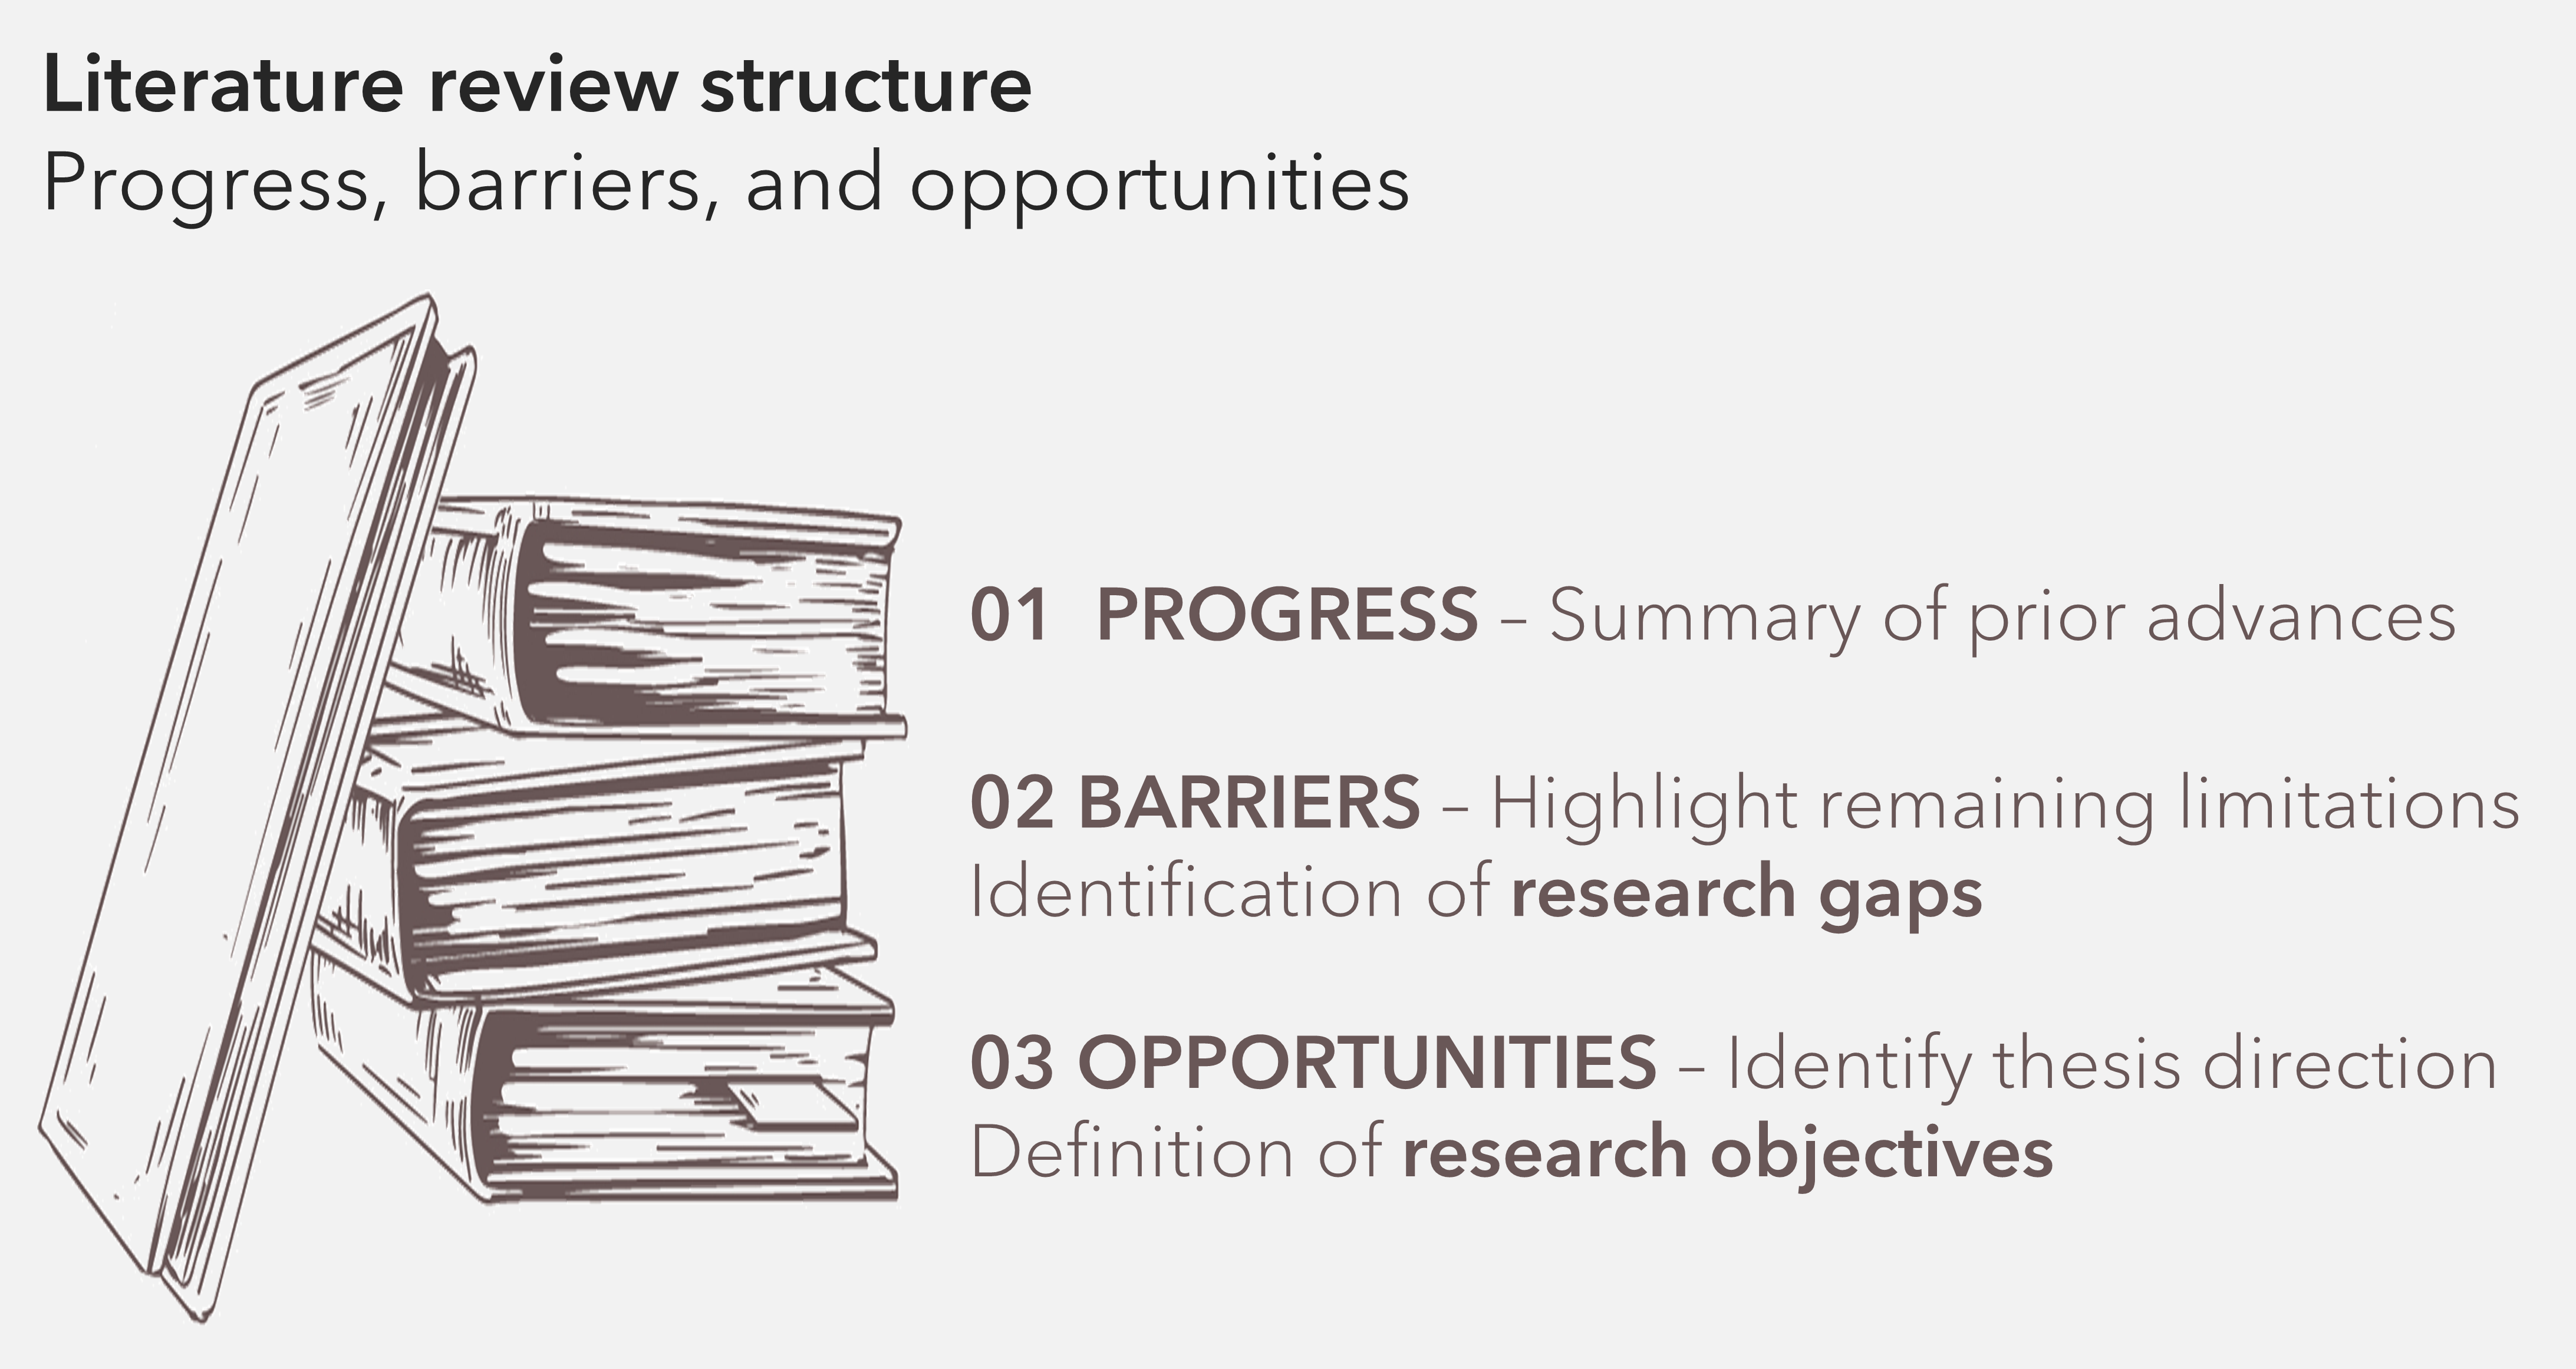
\includegraphics[scale=1.1]{Figures/Chapter_02/literature_structure.png}
\caption{\textbf{Structure of the literature review structure}. This infographic illustrates the organisation of the literature review, highlighting the three key sections: Progress, Barriers, and Opportunities. Each section emphasises the thematic flow from past advancements to current challenges and future research directions.}
\label{fig:literature_structure}
\end{figure}

%%%%%%%%%%%%%%%%%%%%%%%%%%%%%%%%%
\section{Theoretical foundations}
%%%%%%%%%%%%%%%%%%%%%%%%%%%%%%%%%

Flash \marginpara{Definition of flash floods} floods are characterised by a rapid hydrological response to intense rainfall events, with runoff timescales ranging from mere minutes to a few hours \citep{Davis2001}. Its definition should clearly emphasise the immediacy and swift onset of flash floods. However, there remains a degree of ambiguity regarding the boundary between flash floods and other types of floods. Common definitions include \textit{floods with high peak discharge and short duration} \citep{Zain2021}, \textit{events occurring within 6 hours of rainfall} \citep{Kobiyama2007}, and \textit{floods rising and falling rapidly with little warning}. Flash floods exhibit diverse characteristics depending on their type and geographic context. They can be categorised as pluvial or riverine, each presenting distinct risks and impacts \citep{Archer2018}. Flash flood characteristics can also vary based on local topography, soil conditions, and human factors. The ambiguity in distinguishing flash floods from other flood types is compounded by geographic diversity and differing environmental circumstances. For instance, flash flood thresholds applicable to British ecosystems may not adequately represent the phenomena observed in semi-arid or mountainous regions \citep{Archer2019}, making a single, standardised definition challenging to establish. Efforts to establish a unified flash flood definition are also hindered by the lack of comprehensive, high-quality, long-term datasets across different regions, making it difficult to identify universal thresholds and standardise flash flood characterisation \citep{Kaiser2020, Gourley2013}.

Localised \marginpara{Meteorological factors influencing flash floods} extreme rainfall is the primary meteorological driver of flash floods. Several interrelated meteorological factors contribute to the variability in intensity and spatial distribution of extreme rainfall events. For example, large-scale systems such as fronts, cyclones, and troughs can introduce substantial moisture into a region, creating conditions favourable for heavy rainfall. These systems enhance vertical motion and convective activity, leading to localised intense precipitation \citep{Zanchetta2020}. Moreover, mesoscale convective systems such as squall lines and supercells can dramatically concentrate rainfall over small geographic areas, rapidly overwhelming local hydrological systems \citep{Maddox1979}. While these weather systems interact with local topography, land use, and drainage systems to determine the ultimate severity and impact of flash floods, accurately characterising and predicting localised extreme precipitation intensities at fine spatial scales remains an ongoing challenge due to the complexity of atmospheric processes involved \citep{Maqtan2022}. To address these challenges, researchers are developing advanced forecasting tools and early warning systems that integrate high-resolution rainfall observational networks, km-scale NWP models, and ensemble approaches to quantify uncertainties associated with small-scale weather phenomena and provide more accurate and timely warnings for flash flood events \citep{Msigwa2024, AlRawas2024}.

Catchment \marginpara{Hydrological factors influencing flash floods} characteristics play a crucial role in determining the hydrological response to flash flood events. The morphology, topography, land use, and soil properties of a catchment substantially influence its behaviour during extreme rainfall \citep{Henao2022, Liu2011}. Key factors such as antecedent moisture conditions, soil type, and vegetation cover are essential for evaluating runoff generation \citep{Henao2022a, Liu2011}. The scale and size of catchments add complexity to hydrological responses, with larger catchments exhibiting greater heterogeneity in their hydrodynamic behaviours \citep{Luong2021}. Catchment topography significantly modifies water movement patterns, with steeper slopes promoting quicker runoff travel times and concentrated flow pathways \citep{Liu2011, Maqtan2022a}. Soil moisture and infiltration rates are critical hydrological factors governing the occurrence and intensity of flash floods. Initial soil moisture conditions directly influence runoff generation through their effect on infiltration capacities and connectivity between surface and subsurface flow pathways \citep{Yatheendradas2008}. Flash flood forecasting systems rely heavily on accurate initial soil moisture estimates to simulate hydrological responses effectively \citep{Yatheendradas2008, AlRawas2024, Xing2019a}. Uncertainty in initial soil moisture assessments remains a challenge due to spatial heterogeneity and temporal variability in environmental factors \citep{Yatheendradas2008, AlRawas2024}. Streamflow dynamics constitute a critical aspect of hydrological factors influencing flash flood behaviour, encapsulating interactions between surface water flow and driving meteorological inputs \citep{Yang2022}. Spatial variability plays an instrumental role in shaping streamflow characteristics, with the heterogeneity of river basins affecting how water converges and accelerates in channels \citep{Zhang2024}. Accurate measurement of streamflow dynamics hinges on advancements in real-time monitoring technologies and the integration of varying data types into computationally demanding hydraulic simulations \citep{Msigwa2024, Barthold2015}. Sediment load carried during flash floods adds complexity by altering hydraulic efficiencies within channels \citep{Kim2011}.

Urbanisation \marginpara{Anthropogenic factors magnifying flash flood impacts} and land use changes significantly amplify flash flood impacts by altering hydrological processes. Expanding urban areas replace natural landscapes, such as forests, wetlands, and agricultural zones, with impermeable surfaces like roads and pavements, severely reducing the land's capacity to absorb rainfall and thus increasing runoff during extreme precipitation events \citep{Liu2011, Amponsah2018, Saad2024}. The uncontrolled expansion of urban centres frequently leads to inadequate stormwater infrastructure and improper urban planning, increasing vulnerability to severe inundation \citep{Saad2024, Xing2019a}. Moreover, construction in hilly regions destabilises slopes through excavation and soil compaction, accelerating runoff and increasing the risk of landslides during heavy rainfall \citep{Hinge2024}. To mitigate these effects due to urbanisation, strategies must integrate sustainable planning practices alongside flood-resilient infrastructure development. Understanding how hydrological modelling can account for land-use alterations is crucial for improving prediction accuracy and preparedness measures in affected regions \citep{Martinaitis2023}. Adaptive solutions targeting urban settings - such as real-time forecasting systems informed by rainfall variability - can aid local authorities in minimising disaster impacts while ensuring public safety during emergent conditions \citep{Msigwa2024}\citep{Maqtan2022}. Deforestation, particularly prevalent in tropical regions, further exacerbates flood hazards by weakening soil structures, reducing water retention, and intensifying soil erosion \citep{Hinge2024}. This erosion can block drainage channels, diminishing their effectiveness during storms. Similarly, intensive farming practices compact soils, hindering infiltration and enhancing flood severity and frequency. Deforestation also disrupts natural mechanisms for regulating water flow. The loss of tree cover diminishes rainfall interception and accelerates erosion, consequently increasing runoff into rivers and drainage systems beyond their capacities. In Malaysia's West Coast region, rapid urbanisation and deforestation have notably escalated flash flood occurrences, transforming moderately flood-prone areas into severe flooding hotspots. Additionally, sediment transport processes in rivers are disrupted, further intensifying downstream flooding. Even moderate rainfall can trigger severe flooding in areas where forests have been cleared, due to compromised soil stability and impaired water retention. Regions where forests have been replaced by fragmented vegetation experience amplified risks even with relatively low-intensity rainfall. Simple alterations in land use practices can magnify the severity of flash floods by promoting uncontrolled sediment mobilisation while creating conditions conducive to rapid surface water concentration \citep{Kuksina2020}. Interconnected elements - from degraded soil quality to elevated flow velocities - highlight the cascading nature of deforestation-related impacts on flooding dynamics. Geographic features significantly influence flash flood dynamics. Variations in elevation, slope, and terrain shape dictate the severity and distribution of floods. Steep slopes in mountainous terrains promote rapid runoff, increasing sediment transport, flood magnitude, and reducing lag time between precipitation occurrence and flooding \citep{Pham2020, Hinge2024}. Moreover, steep slopes can accelerate water velocity in streams or rivers during a flash flood event, increasing sediment transport and debris flow that may damage infrastructure downstream \citep{Borga2019}\citep{Flamig2020}. Low-lying valleys and depressions, often convergence points for runoff, experience enhanced flood risks due to accumulated moisture from higher elevations \citep{Luong2021}\citep{AlRawas2024}. Additionally, these areas face amplified risks due to topographic wetness caused by accumulated moisture from upstream catchments, magnifying both soil saturation levels and flood severity over time \citep{Hinge2024}\citep{Luong2021}. Urbanisation and deforestation intensify these topographical vulnerabilities by altering natural drainage patterns and decreasing soil permeability. This feedback loop between degraded ecosystems and heightened hydro-meteorological extremes compounds challenges faced when modelling flash flood events accurately across diverse geographical domains. These elements influence hydrological and meteorological processes, thereby increasing the intensity and destructiveness of flash floods. Climate change compounds these issues by altering rainfall patterns and increasing the intensity and variability of precipitation events, which, combined with urban sprawl and deforestation, expand flood-prone zones and magnify flood impacts globally.


%%%%%%%%%%%%%%%%%%%%%%%%%%%%%%%%%%%%%%%%%%%%%%%%%%
\section{Existing flash flood forecasting systems}
%%%%%%%%%%%%%%%%%%%%%%%%%%%%%%%%%%%%%%%%%%%%%%%%%%

Flash \marginpara{The historical evolution of flash flood forecasting systems} flood forecasting has evolved dramatically over the decades, transforming from basic hydrological calculations to sophisticated AI-powered prediction systems that save countless lives worldwide. For example, the global coverage of flash flood guidance systems now serves nearly 3 billion people across more than 60 countries \citep{Georgakakos2021}. The foundations of flash flood forecasting were established through fundamental hydrological concepts developed in the mid-20th century. The unit hydrograph principle became a cornerstone concept for understanding how rainfall translates into streamflow in small watersheds \citep{Rigon2016}. These early approaches relied primarily on mathematical representations of watershed behaviour, with limited data collection capabilities and processing power. Early forecasting methods depended heavily on ground-based observations using in situ sensors, which provided relatively limited spatial coverage and temporal resolution \citep{Tao2024}. During this period, hydrologists developed theoretical frameworks that enabled more sophisticated forecasting. Concepts like lag time, storage, and the geomorphological unit hydrograph emerged as critical tools for understanding the timing and magnitude of flood responses \citep{Rigon2016}. These approaches were mostly applied to larger river systems with longer response times, leaving flash flood prediction, characterised by rapid onset and localised impacts, as a particularly challenging problem for forecasters. The late 20th century saw increasing efforts to translate theoretical hydrological understanding into operational forecasting systems. This period was characterised by growing recognition of flash floods as a distinct hydrological hazard requiring specialised prediction approaches. Early warning systems during this era were primarily deterministic, using rainfall observations and simple rainfall-runoff models to predict potential flooding \citep{Hapuarachchi2011}. As computational capabilities improved in the 1980s and 1990s, more sophisticated hydrological models began to emerge. However, these early systems were limited by data availability, computational constraints, and a lack of integration between meteorological and hydrological forecasting components. Despite these limitations, they represented important steps toward developing dedicated flash flood prediction capabilities \citep{Hapuarachchi2011}.

The \marginpara{Modern flash flood forecasting systems} beginning of the 21st century marked a pivotal moment in flash flood forecasting. A key innovation in modern flash flood forecasting systems has been their ability to integrate diverse data sources. These systems incorporate remotely-sensed precipitation data from geostationary and polar orbiter satellite platforms, reflectivity data from weather radar systems, and ground-based automated precipitation gauge measurements. This multi-source approach helps overcome the limitations of any single data type and provides more robust precipitation estimates, which are the most critical input for flood forecasting. The systems also evolved to include mesoscale NWP model forecasts integrated with land-surface model responses, enabling longer-term guidance products beyond the immediate forecast window. This integration of atmospheric and hydrologic modelling represented a significant advance over earlier, more compartmentalised approaches to flood prediction. The technological revolution has also played an important role in developing operational flash flood forecasting systems. As computational demands for flood forecasting increase, high-performance computing clusters become essential infrastructure for operational systems. For example, a parallel flood forecasting and warning platform, based on high-performance computing clusters, was established in China, enabling nationwide coverage with particular effectiveness for flash flood prediction. This platform utilises advanced file-based message passing on a shared hierarchical storage system, pre-allocation and dynamic allocation methods for resource management, and automatic switching between different time-scale models driven by rainfall events. These computational advances allowed for unprecedented spatial and temporal resolution in modelling, enabling more localised and accurate predictions. The ability to process vast quantities of data in near-real-time transformed the capabilities of forecasting systems, substantially reducing the gap between observation and warning issuance.


%%%%%%%%%%%%%%%%%%%%%%%%%%%%%%%%%%%%%%%%%%%%%%%%%%%%%%%%%%%%%%%%%%%%%%%%
\subsection{Flash flood forecasting systems characterisation by model's spatial domains}

Urban \marginpara{Urban flash flood forecasting systems} flash flood forecasting requires specialised approaches due to complex city environments with varied land use, impermeable surfaces, and intricate drainage systems. Traditional channel models often fail to capture localised ponding scenarios independent of river overflow. Challenges include predicting pluvial flash floods, where rainfall directly generates surface runoff without channel interaction, and insufficient integration of socioeconomic vulnerability data. Innovations include high-resolution DEMs, real-time IoT sensor networks, machine learning algorithms, and ensemble precipitation modelling. Future systems must integrate hydrological observations with meteorological forecasts and regional thresholds to improve prediction accuracy in expanding urban landscapes. 

Regional \marginpara{Regional and national flash flood forecasting systems} and national forecasting systems are vital in enhancing localised flash flood prediction capabilities. These systems are designed to address the specific geographic, climatic, and infrastructural conditions of their host countries or regions. By leveraging global data inputs and incorporating locally sourced datasets, they refine predictions and improve actionable outputs. The Cascading Forecasting Process, utilised within frameworks such as the Southern Africa Severe Weather Forecast Demonstration Project (SWFDP), exemplifies this approach. It facilitates the transfer of forecast outputs from advanced global centres to designated regional hubs, which interpret and provide guidance on imminent severe weather events \citep{Jubach2016}. Effective regional systems rely heavily on local ownership and accessibility of input data, often maintained under specific agreements by hydro-meteorological agencies or related institutions. This underscores the importance of robust inter-institutional collaboration \citep{Georgakakos2022}. Despite advancements in spatial resolution, adaptability, and probabilistic approaches \citep{Zanchetta2020, AlRawas2024}, challenges persist in less monitored areas where gauging stations are sparse \citep{Kuksina2020}. Addressing these observational gaps while maintaining fidelity across models tailored to specific catchments is crucial for system resilience due to climatic variability and infrastructure limitations \citep{Liu2011, Douinot2016}. 



%%%%%%%%%%%%%%%%%%%%%%%%%%%%%%%%%%%%%%%%%%%%%%%%%%%%%%%%%%%%%%%%%%%%%%%%
\subsection{Flash flood forecasting systems characterisation by model output's uncertainty}

Deterministic \marginpara{Deterministic models} models play a crucial role in flash flood forecasting by predicting outcomes based on fixed inputs and mathematical formulations. These models simulate physical processes such as precipitation, runoff generation, and soil infiltration. However, their specificity and rigidity pose challenges when dealing with the complexity of natural systems \citep{AlRawas2024, Liu2018}. Deterministic approaches struggle with representing probabilistic uncertainties associated with extreme localised rainfall events. Grid-based deterministic systems integrate diverse datasets to provide location-specific forecasts, but uncertainties tied to erroneous rainfall estimates can magnify errors within smaller basins \citep{Yatheendradas2008, Msigwa2024}. Advancements in objective algorithms and combined approaches like Warn-on-Forecast systems (WoFS) and Probabilistic Flooded Locations modules (PRO-FLASH) aim to improve performance \citep{AlRawas2024}. However, evolving real-world phenomena introduce significant prediction variabilities across longer operational timelines \citep{Pham2020, AlRawas2024}. Integrating multi-source observational data at increasing spatial scales can enhance adaptability while resolving precision discrepancies in deterministic calibrations \citep{Lu2021, Liu2018}. 

Probabilistic \marginpara{Probabilistic models} models are, therefore, essential in flash flood forecasting due to their ability to address inherent uncertainties in meteorological and hydrological predictions. Using ensemble simulations with varying initial conditions or parameter sets, probabilistic approaches generate various possible outcomes, quantifying the uncertainty associated with forecasted flash flood risks \citep{Yang2022}. Ensemble-based probabilistic precipitation forecasts derived from Ensemble Prediction Systems (EPS) allow for improved characterisation of rainfall forecast uncertainties. However, these systems require significant computational resources, hindering their practical implementation in regions with limited technological infrastructure \citep{Poolman2014}. Coupling ensemble quantitative precipitation forecasts (QPFs) with hydrologic models designed for flash flood forecasting has led to advancements such as sub-hourly flash flood guidance \citep{Martinaitis2023, Barthold2015}. Probabilistic hydrologic ensembles capture spatio-temporal variations across diverse terrains, offering more adaptability than deterministic counterparts when addressing localised extreme rainfall scenarios \citep{Filho2021}. Despite the promise of probabilistic frameworks, challenges remain in integrating real-time data streams and visualising probability distributions effectively \citep{Alfieri2015, AlRawas2024}. Nonetheless, ongoing initiatives continue to advance the efficacy of flash flood early warning systems (FFEWS) by enhancing decision reliability during critical lead-time gaps, ensuring scalability across diverse environmental and socioeconomic contexts worldwide \citep{Yang2022, Zanchetta2020}.

%%%%%%%%%%%%%%%%%%%%%%%%%%%%%%%%%%%%%%%%%%%%%%%%%%%%%%%%%%%%%%%%%%%%%
\subsection{Flash flood forecasting systems characterisation by model implementation}

Physical \marginpara{Physical models} models are a critical component of flash flood forecasting systems, employing principles derived from physical laws and equations to simulate hydrological processes. These models capture the intrinsic behaviour of natural processes such as precipitation-runoff transformations, soil infiltration, and river routing without relying on statistical or empirical relationships \citep{Hinge2024}. Operational systems like the Ensemble Framework For Flash Flood Forecasting (EF5) incorporate physical models to produce actionable runoff predictions while maintaining computational feasibility \citep{Flamig2020}, and their scalability allows for iterative improvements and parameter adjustments across diverse spatial domains \citep{Xing2019a}. Physical modelling intersects with uncertainty quantification frameworks, such as ensemble-based methods or probabilistic estimations, and systems like Flood-PROOFS utilise downscaling techniques to refine deterministic weather predictions into high-resolution forecasts for flash flood risk evaluation \citep{Zanchetta2020}. Challenges persist in achieving universality due to varying regional requirements and climatic patterns \citep{Xing2019a, AlRawas2024}. However, application frameworks like FLASH leverage ensemble configurations and physically-derived parameters to assimilate real-time meteorological inputs accurately, improving lead times for emergency alerts \citep{Martinaitis2023}. Despite the complexities associated with implementation, physical models remain indispensable in advancing global flash flood forecasting capabilities by simulating hydrological interactions through theoretical foundations rooted in science \citep{Jubach2016, Zanchetta2020, AlRawas2024, Martinaitis2023}. 

Data-driven \marginpara{Data-driven models} models have gained prominence in flash flood forecasting due to their ability to leverage large datasets and identify complex patterns in meteorological and hydrological variables. These models employ statistical, machine learning, or neural network techniques to predict flash flood occurrences and associated risks based on historical and real-time data. A notable example is the Data-Driven Hydrological Model (DaHM), which uses a feed-forward two-layer perceptron architecture to capture non-linear relationships between input variables like precipitation and streamflow \citep{Philipp2016}. Data-driven frameworks offer the advantage of relying on empirical data rather than explicitly defined physical equations, enabling a broader range of applications where observational data is abundant \citep{Zanchetta2020, Msigwa2024}. However, their robustness is tied to the availability and quality of input datasets, and challenges arise in regions with limited historical records or sparse monitoring networks \citep{Zanchetta2020, Lu2021}. Despite inherent uncertainties in predicting localised extreme rainfall events, data-driven models continue to evolve by combining traditional observational techniques with machine learning components \citep{AlRawas2024}. Coupling data-driven models with physics-based frameworks leverages the strengths of both paradigms, fostering improvements in predictive skill and actionable knowledge dissemination \citep{Msigwa2024}. As emerging models develop under expanding computational power and integrated datasets, there is a need for standardised benchmarking across different geographies. Research gaps persist regarding the length and fidelity of archived records essential for training algorithms appropriately \citep{Zanchetta2020}. Ongoing research focuses on improving scalability without sacrificing accuracy amid increasingly variable climatic influences driven by global environmental changes \citep{AlRawas2024, Lu2021}.


%%%%%%%%%%%%%%%%%%%%%%%%%%%%%%%%%%%%%%%%%%%%%%%%%%%%%%%%%%%%%%%%%
\section{Current challenges in achieving medium-range flash flood predictions over a continuous global domain}
%%%%%%%%%%%%%%%%%%%%%%%%%%%%%%%%%%%%%%%%%%%%%%%%%%%%%%%%%%%%%%%%%

Despite significant advancements in forecasting technologies, observational capabilities, and computational resources, developing a global flash flood forecasting system capable of producing medium-range predictions over a continuous domain remains an ongoing challenge. The primary obstacle lies in the inherent difficulties of accurately predicting extreme localised rainfall events - the main drivers of flash floods - as the small-scale atmospheric processes responsible for such localised extreme rainfall events are challenging to represent in km-scale and global NWP models. Furthermore, the rapid evolution and short-lived nature of flash floods, combined with the intricate interplay between meteorological, hydrological, and anthropogenic exacerbating factors, pose additional hurdles in achieving timely and precise forecasts on a global scale. While existing systems have demonstrated success in specific regions or at shorter lead times, extending these capabilities to a unified, worldwide framework requires addressing several critical research gaps and overcoming technical and logistical barriers.


%%%%%%%%%%%%%%%%%%%%%%%%%%%%%%%%%%%%%%%%%%%%%%%%%%%%%%%%%%%%%%%%%%%
\subsection{Challenge n.1: evaluate predictions of localised extreme rainfall up to medium-range lead times over a continuous global domain}

Historically, heavy rainfall forecasts have been verified against observed precipitation, under the implicit assumption that improving quantitative precipitation forecasts (QPF) will directly improve flash flood prediction \citep{Herman2018}. Most operational flash flood guidance systems rely on rainfall threshold exceedance to infer flood risk \citep{Georgakakos2006}, essentially using precipitation as a proxy for flash floods. While this assumption is logical (extreme rainfall is a primary driver of flash floods), it has seldom been rigorously tested at a global scale \citep{Herman2018}. Verifying forecasts against actual flash flood occurrences (as reported in impact databases or hydrological observations) is complicated. Flash floods are binary events (either occurring or not in a given area and time), whereas NWP provides continuous rainfall fields. There is an inherent mismatch in comparing these dissimilar quantities. Direct, “impact-based” verification frameworks have been proposed to address this gap by evaluating how well rainfall forecasts correspond to documented flash flood events \citep{Ntelekos2006,CharpentierNoyer2023}. Such approaches move beyond rainfall-to-rainfall verification, but they face significant methodological hurdles.

A major challenge in flash-flood-focused forecast verification is defining appropriate metrics. Standard continuous metrics (e.g., mean error, correlation) are not meaningful for rare binary (yes-/no-) events, and even traditional contingency table scores (probability of detection, false alarm ratio, etc.) must be interpreted with care for highly localised phenomena \citep{Hapuarachchi2011}. Moreover, the lack of standardised, flash-flood-specific verification metrics has hindered comparison across studies and regions \citep{CharpentierNoyer2023}. Different researchers have adopted a variety of performance measures. For instance, \citet{CharpentierNoyer2023} used event-based receiver-operating characteristic analyses for threshold exceedances of streamflow to evaluate flash flood predictions, whereas \citet{Viterbo2020} combined object-based, grid-based, and point-based verification approaches to assess a particularly extreme flash flood event. Such multi-criteria verification highlights that no single metric can capture all aspects of flash flood forecast performance (timing, location, intensity) \citep{Viterbo2020}. There is a clear need for a coherent framework tailored to flash flood forecasting, blending metrics from meteorology and hydrology.

Another difficulty lies in the spatial and temporal uncertainties of both forecasts and observations. Flash floods typically occur on very small scales (a few $\mathrm{km}^2$) and within short cloudburst durations, whereas even the highest-resolution global models (grid spacing on the order of 9--13~km) only parameterise convection, producing rainfall smoothed over large grid boxes \citep{Hewson2021}. This scale mismatch means that a model may predict heavy rainfall in the general vicinity of an event but miss the exact location or timing critical for an accurate warning \citep{Collier2007}. Traditional grid-point verification will then penalise the forecast (the so-called “double penalty” problem), even if it correctly captures the broader scenario of convective activity. To address this, “fuzzy” or neighborhood verification methods have been advocated, allowing spatial and temporal tolerances when matching forecast rainfall to flash flood observations \citep{CharpentierNoyer2023}. For example, an observed flash flood might be matched with a forecast that predicted an extreme rainfall cell a short distance away or a few hours off, acknowledging inherent position errors in NWP. Developing scale-appropriate verification techniques is essential to fairly evaluate global model skill in this context.

Data scarcity and reporting biases further complicate verification efforts. Flash flood impacts are often under-reported, especially in remote regions, making it difficult to compile reliable “truth” data for verification \citep{Hapuarachchi2011}. Global disaster databases tend to record only the most severe events, so many smaller-scale flash floods go undocumented. This can lead to false alarms in an impact-based verification (a forecast might correctly predict a heavy downpour capable of causing a flash flood, but no official report exists to confirm the event). Conversely, some reported flash floods may be missing or mis-timed relative to the causative rainfall. Efforts to improve observational data include integrating ground reports with remote sensing (radar, satellite) and even crowdsourced information to build more comprehensive flash flood catalogues \citep{Pham2020}. Nonetheless, any verification framework must account for uncertainty in the observations. \citet{Ntelekos2006} highlighted the need for probabilistic approaches to flash flood guidance, partly to reflect uncertainty in whether a given rainfall event will translate to an actual flood. In practice, a verification exercise might incorporate an ensemble of observed outcomes (e.g., treating unreported events as possible misses) or apply a penalty for missed reports. These strategies remain an active research area as scientists strive to quantify forecast skill given imperfect observations.

Despite these challenges, there is evidence that global NWP forecasts can provide useful guidance for flash flood risk, especially when enhanced with post-processing and ensemble techniques. Modern global models are capable of predicting the synoptic and mesoscale conditions that lead to convective extremes (such as moisture surges, atmospheric instability, and triggering fronts or orography). The predictability horizon for specific convective events is inherently limited (often a few days at best) \citep{Collier2007}, but ensemble forecasting offers a way to express flash flood risk probabilistically. For example, the U.S. Weather Prediction Centre’s Excessive Rainfall Outlook uses global ensemble QPF to indicate probabilities of rainfall exceeding flash flood thresholds out to several days. Similarly, when statistically downscaled, the European Centre’s ensemble forecasts have demonstrated skill in highlighting localised extreme rainfall events up to around 10 days in advance \citep{Hewson2021}. One such post-processing approach, “ecPoint”, stochastically adjusts coarse-grid rainfall predictions to account for sub-grid variability, significantly improving the representation of localised extreme rainfall events \citep{Hewson2021}. \citet{Hewson2021} showed that the probabilistic forecast of point rainfall extremes from a global ensemble can be extended to the medium range with increased reliability and discrimination ability, especially for extreme events, which is crucial for early flash flood warnings. In a recent proof-of-concept study in the Andes, a post-processed global forecast successfully pinpointed a flash-flood-producing storm that the raw model rainfall field had underestimated, illustrating the potential benefits of tailored post-processing in identifying flash flood risks \citep{Herman2018}.

Table~\ref{tab:ff_challenges} summarises key challenges identified in the literature for forecasting and verifying flash floods using global model outputs, along with proposed strategies to address them. These challenges span from data limitations to methodological issues in translating model forecasts to actionable flood risk information. While ongoing research is making progress in each area, effectively outrunning flash floods --- i.e., providing timely and accurate warnings --- will likely require an integrated approach that combines improved NWP, clever post-processing, and dedicated flash-flood-specific verification frameworks.

\begin{table}[hbt]\centering
\caption{Key challenges in using global NWP rainfall forecasts for flash flood risk identification, and proposed solutions from recent studies.\label{tab:ff_challenges}}
\begin{tabular}{p{4.5cm} p{6.2cm} p{5.5cm}}
\hline
\textbf{Challenge} & \textbf{Impact on Forecast Reliability} & \textbf{Proposed Solutions} \\
\hline
Data limitations (sparse gauges, under-reporting of flash floods) & Missed or mischaracterized events in verification datasets; difficulty in model calibration & Integrate multiple data sources (radar, satellite, crowdsourcing) for event detection \citep{Pham2020}; rigorous quality control of impact databases \\
Spatial-scale mismatch between global model output and local flood processes & Forecast rainfall may not resolve flash-flood-scale intensity or timing, reducing predictive accuracy & Higher-resolution nested models or convection-permitting ensembles for hotspots \citep{Vincendon2011} (e.g. Mediterranean basins); scale-aware verification (neighborhood methods) to allow positional uncertainty \citep{CharpentierNoyer2023} \\
Verification framework (metrics and methods) & Standard metrics may not capture flash flood event performance, hindering model comparison & Develop flash-flood-specific metrics and multi-criteria evaluation (e.g., event-based ROC, peak timing error) \citep{CharpentierNoyer2023,Viterbo2020}; verify forecasts against impacts (impact-based verification) \citep{Herman2018} \\
Uncertainty quantification & Deterministic forecasts can be overconfident for rare events, missing low-probability extreme scenarios & Use ensemble forecasting and probabilistic thresholds for flood guidance \citep{Ntelekos2006}; perturbation methods to generate scenario ensembles \citep{Vincendon2011} \\
Model representation of land surface \& hydrology & Inaccurate initial soil moisture or runoff schemes can misestimate flood triggering & Couple NWP with hydrological models for flash flood prediction; adjust for antecedent conditions or use machine-learning surrogates (ongoing research) \\
\hline
\end{tabular}
\end{table}

In summary, global NWP rainfall forecasts have an important role in identifying flash flood risks, but realising their full potential requires overcoming significant verification and modelling challenges. Literature to date suggests that while raw global models alone only partially succeed in pinpointing flash flood events, their performance improves markedly with specialised post-processing, ensemble prediction, and impact-based evaluation techniques. By developing verification frameworks that directly address flash flood occurrences (rather than just rainfall error) and by incorporating uncertainty and high-resolution information, researchers are moving closer to answering RQ1. The insights gained here form a foundation for exploring new complementary approaches. In particular, the limitations of physics-based models in forecasting flash floods motivate the investigation of data-driven methods, which is the focus of the next section of this review.

%%%%%%%%%%%%%%%%%%%%%%%%%%%%%%%%%%%%%%%%%%%%%%%%%%%%%%%%%%%%%%%%%%%%%%
\section{Challenge n.2: assess the feasibility of data-driven flash flood prediction using reanalysis data}

Data-driven approaches are increasingly being explored for flash flood forecasting, with the aim of overcoming limitations of traditional physics-based methods in data-sparse regions, as stated in the previous section. Recent reviews indicate that a majority of flash flood prediction studies now incorporate machine learning or artificial intelligence techniques \citep{AlRawas2024}, reflecting a shift toward data-driven modelling. This section examines the feasibility of developing a global flash flood prediction system using hydro-meteorological reanalysis data as inputs. Key considerations include the selection of predictive features, the scarcity and quality of historical flash flood observations, suitable model architectures, uncertainty quantification, and the computational trade-offs inherent in operationalising such a system. By leveraging global reanalysis datasets (e.g., ERA5) and advanced modelling, data-driven flash flood forecasts promise to extend warning lead times and coverage to underserved regions, aligning with initiatives to provide early warnings for all communities. The following subsections discuss the opportunities and challenges in realising this potential. 

\subsection{Data Availability and Feature Selection} Global atmospheric reanalysis products offer a consistent, spatially extensive record of hydro-meteorological variables that can be exploited for flash flood prediction. Modern reanalyses such as ERA5 provide hourly estimates of precipitation, soil moisture, temperature, and other land-surface conditions at $\sim$30km resolution worldwide \citep{Hersbach2020}. These datasets can serve as primary inputs (predictor features) for data-driven models, in lieu of sparse ground observations. The principal driving factor for flash floods is intense short-duration rainfall, so precipitation variables from reanalysis are of foremost importance. However, simply using raw precipitation as a predictor may be insufficient. Studies show that flash flood occurrence depends not only on rainfall intensity, but also on rain event duration and spatial extent, as well as catchment predisposition \citep{Hapuarachchi2011}. For instance, an analysis in Europe found that extreme rain events which induced flash floods tended to last longer and cover larger areas than those that did not cause flooding, even if peak intensities were similar \citep{Bronstert2021}. Accordingly, features such as accumulated rainfall over various durations (e.g. 1h, 3h, 6h, 12h, and 24h totals), rainfall intensity thresholds, and storm footprint area can enhance predictive skill by characterising the critical rainfall volume and concentration that trigger flash floods. In addition to precipitation, it is vital to include antecedent and catchment-condition indicators as features. Flash flood generation is modulated by soil moisture and land surface properties that control infiltration and runoff. Traditional flash flood guidance systems compute rainfall thresholds based on soil saturation and hydrologic response \citep{Georgakakos2022}. Emulating this, data-driven models can ingest proxy variables for catchment wetness, such as antecedent precipitation indices (cumulative rainfall in days prior) or direct soil moisture estimates from reanalysis or remote sensing. Topographic and land cover attributes are also important static features: high-resolution elevation data (slope, basin area, drainage density) and land use (impervious cover) influence runoff rates. These attributes can be combined with meteorological inputs to improve model generalisation across diverse terrains. For example, \citet{Alkaabi2025} incorporate a digital elevation model with ERA5 rainfall and runoff data to predict flash-flood runoff in an arid watershed, allowing the model to learn the influence of terrain on flood response. Likewise, global catchment datasets (e.g., CAMELS) provide physiographic descriptors used as additional inputs in large-sample hydrological models \citep{Kratzert2019}. Selecting a rich set of features that capture both the triggering hazard (extreme rainfall) and the susceptibility of the landscape (storage and runoff capacity) is therefore crucial for a data-driven flash flood predictor. Reanalysis products offer many of these features globally, but their coarse resolution poses a challenge: flash floods often occur at scales ($<100~\text{km}^2$) smaller than a reanalysis grid cell, potentially smoothing out critical localised extremes. This scale mismatch motivates either downscaling of reanalysis data or inclusion of higher-resolution data (e.g., satellite cloud products or terrain corrections) to resolve convective storm dynamics. Overall, the global availability of reanalysis variables covering atmospheric and land surface conditions makes them an attractive data source, but careful feature engineering is required to ensure that key predictors of flash flooding are represented despite resolution limitations.

\subsection{Data Scarcity and Event Documentation} 
A fundamental hurdle in developing data-driven flash flood models is the scarcity of reliable historical event data for model training and validation. Flash floods are relatively infrequent and highly localised, and unlike river floods, they often occur in ungauged basins with no stream gauge records of discharge or water level. Many flash flood events are documented only anecdotally (e.g., through post-event reports, disaster databases or news media) or via indirect observations (damage reports, remote sensing of flood aftermath). This leads to a paucity of labelled examples for supervised learning. The limited sample of flash flood occurrences also introduces a strong class imbalance: most time steps and locations correspond to “no flash flood” conditions, which can bias a model unless special training strategies are adopted. Some regions have assembled flash flood event catalogues — for instance, the U.S. and Europe maintain databases of flash flood reports — but globally, there is no unified flash flood archive with consistent reporting criteria. Modellers must therefore integrate heterogeneous data sources or use proxies to identify flash flood events in historical records. One feasible approach is to leverage reanalysis-driven hydrological simulations as a substitute for direct observations of flash flooding. \citet{Alkaabi2025} demonstrate this strategy in a data-sparse desert catchment: they first validated ERA5-derived runoff against a calibrated hydrologic model (HEC-HMS) for past storm events, then used the reanalysis precipitation-runoff pairs to train a deep learning model for flash flood runoff prediction. By doing so, they generated a training dataset from reanalysis that mimics the catchment’s flood response without extensive gauged flow data. Another example is the use of global runoff models or flood reanalysis products (e.g., GloFAS reanalysis) to identify periods of extreme flow that correspond to flash flooding conditions \citep{Wu2022}. While these proxies are imperfect – hydrologic models have their uncertainties – they can considerably expand the training sample size. Additionally, remote sensing offers emerging means to detect flash flood impacts (e.g., sudden increases in river turbidity or soil wetness observable by satellites), which could infer flash flood occurrences in ungauged basins for model training \citep{Smith2021}. Despite such innovations, the challenge of limited ground truth data remains a central issue for global flash flood prediction feasibility. It is difficult to capture the full spectrum of flash flood phenomena (from minor inundations to catastrophic torrents) with coarse datasets. Many events, especially in remote regions, may go unrecorded, leading to under-reporting bias. Models trained only on recorded events might struggle to predict floods in regions with no history in the dataset, even if physical conditions are ripe for flooding. Data augmentation and transfer learning become important in this context: by training on diverse climates and geographies, a model may learn general patterns that transfer to ungauged locations. Recent work in hydrology has shown that deep learning models can indeed extrapolate to ungauged basins by exploiting large training samples and catchment descriptors \citep{Kratzert2019, Gilon2024}. However, those efforts have primarily addressed riverine floods; flash floods pose additional complexity due to their rapid onset and small spatial scale. In summary, assembling a representative and extensive training dataset for global flash flood prediction is non-trivial. It likely requires combining multiple data sources (reanalysis, remote sensing, simulated events, and whatever observational records exist) to capture both positive cases (flash flood occurrences) and negatives (similar meteorological events that did not cause flooding). Careful curation of such a dataset is critical to the feasibility of any data-driven flash flood model. 

\subsection{Modelling Approaches and Architectures} 
The choice of modelling architecture plays a pivotal role in capturing the nonlinear relationships between meteorological inputs and flash flood occurrence or magnitude. A range of machine learning techniques has been explored in recent literature, from relatively simple classifiers to advanced deep learning networks. Statistical and tree-based models have been used at one end of the spectrum to estimate flash flood susceptibility. For example, \citet{Saber2022} applied gradient-boosted decision trees (LightGBM and CatBoost) to identify flash flood-prone catchments in arid regions. These models used geomorphological and climatic predictors to classify areas by flood risk, achieving high accuracy in delineating susceptible zones. While such approaches are interpretable and computationally efficient, they typically operate in a static or event-based context (e.g., producing a susceptibility map) rather than forecasting an imminent flood given real-time inputs. Sequence-based models are more appropriate for dynamic flash flood prediction on short lead times. Recurrent neural networks (RNNs) like the Long Short-Term Memory (LSTM) have been successfully employed to forecast river discharge in flash-flood-prone basins based on time series of rainfall inputs \citep{Song2020}. LSTM models can learn temporal dependencies (e.g., how antecedent rainfall influences current runoff) and have shown better performance than traditional hydrological models in some cases \citep{Song2020}. Building on this, researchers have developed hybrid deep learning architectures to incorporate spatial information as well. Convolutional Long Short-Term Memory networks (ConvLSTM), which blend CNNs and RNNs, allow modelling of both spatial and temporal patterns in the data. \citet{Oddo2024} present a ConvLSTM-based model that ingests multi-modal remote sensing and in-situ data (e.g., gridded rainfall fields, soil moisture, and river stage measurements) to predict flash flood stream levels in a small watershed. By learning the spatio-temporal evolution of storms and catchment response, the ConvLSTM achieved approximately 26\% reduction in prediction error compared to a standard LSTM, effectively capturing localised flood dynamics that the purely temporal model missed \citep{Oddo2024}. This underscores the potential of deep networks to improve flash flood forecasts by recognising spatial rainfall patterns (such as movement and intensity distribution of convective cells) that lead to rapid runoff concentration. Model architecture must also balance generality and specialisation in a global prediction setting. A single model could be trained with data from many regions to learn universal relationships, as was done by \citet{Gilon2024} for global river flood forecasting using an LSTM-based framework. Alternatively, the modelling framework might allow regional customisation, selecting the best algorithm for each locale. The latter approach was illustrated by \citet{Soares2025}, who developed a machine-learning framework (ML4FF) for flash flood forecasting that can be tailored to different watersheds. In their study on a Brazilian basin, the framework tested multiple algorithms and identified an optimal model for that site, highlighting that no one model type uniformly outperforms others everywhere. This suggests that for a global system, a hierarchy of models might be needed: simpler models (e.g., logistic regression or decision trees) could suffice in some data-rich regions, whereas deep learning might be necessary in complex or data-poor regions to capture subtler patterns. Another promising avenue is hybrid modelling that integrates physical knowledge into data-driven models. For instance, Neural Ordinary Differential Equation (NODE) networks have been used to embed rainfall-runoff process dynamics within a deep learning model \citep{Alkaabi2025}, aiming to improve physical consistency and extrapolative power. Similarly, coupling data-driven components with hydrodynamic models (as in a K-Nearest Neighbours post-processor to a physics-based model \citep{Zhou2023}) has been tried to leverage the strengths of both paradigms. Table~\ref{tab:ffstudies} provides a brief overview of representative studies that have explored data-driven flash flood prediction through various modelling approaches. These examples illustrate the diversity of model types (from tree-based to deep learning) and the range of data sources and scales involved. Taken together, the literature demonstrates that data-driven models \textit{can} learn the complex trigger-response relationships for flash flooding, at least in local or regional settings. The feasibility of scaling these approaches globally will depend on choosing appropriate architectures that can handle diverse conditions. In practice, a combination of approaches might be warranted: for instance, using an LSTM or ConvLSTM as a core global model, augmented by region-specific calibration or an ensemble of models to account for local peculiarities. The flexibility and relatively low computational cost of running trained ML models is an advantage here – it is conceivable to run thousands of small-basin models in parallel across the globe in real time, something that would be computationally prohibitive with process-based simulations for every basin. The challenge lies in achieving robust training for each model (as discussed in the previous subsection on data scarcity) and ensuring that the chosen architectures remain stable and accurate when deployed in new regions or under non-stationary climate conditions. 

\begin{table}[h!]\centering
\begin{tabular}{p{3.5cm}p{3.2cm}p{3.3cm}p{4.5cm}}
\hline
\textbf{Study (Year)} & \textbf{Region/Scale} & \textbf{ML Method} & \textbf{Key Findings} \
\hline
Song et al. (2020) \citep{Song2020} & Mountainous catchments (China) & LSTM neural network & Data-driven LSTM model for short-term streamflow forecasting improved flash flood prediction accuracy over traditional hydrological models in steep basins. \
Saber et al. (2022) \citep{Saber2022} & Arid wadis (North Africa) & LightGBM & CatBoost (ensemble trees) & ML-based susceptibility mapping identified flash-flood-prone areas with high precision (AUC $>$ 0.8), demonstrating the usefulness of terrain and climate features in ungauged basins. \
Oddo et al. (2024) \citep{Oddo2024} & Small watershed (USA) & ConvLSTM (deep learning) & Hybrid ConvLSTM using multi-source rainfall and soil data reduced prediction error by $\sim$26% compared to an LSTM, improving lead time and reliability of flash flood warnings. \
Alkaabi et al. (2025) \citep{Alkaabi2025} & Desert catchment (UAE) & CNN-RNN + Neural ODE & Deep learning model using ERA5 reanalysis rainfall and DEM inputs successfully predicted flash flood runoff, matching a physics-based model’s performance in a data-sparse region. \
Soares et al. (2025) \citep{Soares2025} & Tropical basin (Brazil) & ML framework (multiple models) & Automated framework tested various ML algorithms per watershed; a customized model achieved best results, underscoring that optimal flash flood prediction models may differ by region. \
\hline
\end{tabular}
\caption{Selected studies demonstrating data-driven approaches for flash flood prediction. These examples span different climates and methodologies, from neural networks to tree-based models, highlighting the range of techniques applied to flash flood forecasting problems.}
\label{tab:ffstudies}
\end{table} 

\subsection{Uncertainty Quantification and Model Validation} 
Any feasible flash flood prediction system must grapple with significant uncertainties. Flash floods are inherently difficult to predict with high confidence due to the nonlinear thresholds involved (small changes in storm intensity or location can make the difference between minor flooding and a major flash flood). Data-driven models add additional uncertainty stemming from limited training data and potential model overfitting or bias. It is therefore essential to quantify prediction uncertainty and convey it in early warning contexts. In practice, this might involve producing probabilistic forecasts (e.g., the probability of flash flood occurrence in a given area) rather than deterministic yes/no predictions. Traditional flood forecasting often employs ensemble simulations to characterise uncertainty, but generating large ensembles of a machine learning model is computationally trivial once the model is trained (sample multiple realisations via Monte Carlo dropout or bootstrap aggregating). The larger challenge is calibration and interpretation: ensuring that the model’s probability estimates are reliable and correspond to real-world frequencies. Some initial work in data-driven hydrology has explored methods like quantile regression neural networks to predict not just a single outcome but a distribution of possible outcomes \citep{Zhong2023}. For flash floods, such approaches could yield prediction intervals for peak flow or flood severity, which are valuable for risk-based decision-making. However, these methods have yet to be widely tested in flash flood scenarios, and communicating uncertainty to end-users (e.g., local emergency managers) in an understandable way remains an open issue. 

Another aspect of feasibility is how to rigorously evaluate and validate the performance of a global flash flood ML model. Without standard benchmarks, comparing models can be difficult. Different studies have used a variety of metrics: for instance, flood forecasting evaluations have reported continuous errors like Nash–Sutcliffe Efficiency or RMSE for water level predictions \citep{Oddo2024}, as well as categorical metrics like the probability of detection, false alarm ratio, and area under the ROC curve for flood/no-flood predictions \citep{Saber2022}. The lack of a consistent verification framework means each new model must be carefully tested against multiple criteria. Ideally, a global model would be evaluated on historical flash flood events across diverse regions. In practice, one might validate the model retrospectively by checking whether it would have issued warnings for known past flash floods. \citet{Georgakakos2022} emphasises the importance of such benchmarking: their flash flood guidance system is continually verified using archived rainfall events and reported flash floods to ensure that the system’s thresholds are performing as expected. For a data-driven model, a similar retrospective analysis is needed, potentially using cross-validation by region and by event. One specific pitfall in validation is the quality of “ground truth.” As noted, flash flood observations are often sparse or qualitative. Model false alarms might sometimes be due to errors in observations (a flood may have occurred but was not reported), and model misses could be partly attributable to missed inputs. To build confidence in the model, it may be necessary to supplement conventional validation with case studies and post-event forensic analysis. For example, if the model misses a major flash flood, analysing the event could reveal if the input data failed to capture an extreme local rainfall intensity or if the model did not adequately learn a particular combination of factors. Such insights can guide further improvements (e.g., adding a new feature or expanding training data for that regime). 

\subsection{Computational and Operational Considerations} 
Implementing a data-driven flash flood prediction model on a global scale presents practical considerations in terms of computation, integration, and maintenance. One advantage of data-driven models is their fast runtime once trained: evaluating a machine learning model (even a complex deep network) is typically a matter of milliseconds per grid cell or catchment, which is far faster than running detailed physics-based hydrologic simulations over the same domain. This makes it plausible to generate worldwide flash flood risk forecasts in near-real-time, provided that the required input data (e.g. short-range rainfall forecasts from a numerical weather prediction model or reanalysis updates) are available and can be ingested efficiently. The heavy computation for ML models lies in the training phase, which can be done offline with high-performance computing resources. Training a global model on decades of reanalysis data and flash flood events would indeed be a substantial but one-time (or infrequent) effort. Studies such as \citet{Gilon2024} have shown that training an AI flood model on a global scale is feasible with modern compute infrastructure, having built a model covering 80+ countries. Once deployed, that model ran continuously to provide 5-day flood forecasts, demonstrating the operational viability of a global data-driven system. For flash floods, the data volumes might be even larger (due to higher temporal resolution needed), but still within the reach of current big data technology. On the other hand, the complexity of the model architecture can become a hindrance in operational settings. Simpler models are easier to maintain and update. In a multi-model framework, there is a trade-off between optimal accuracy and manageability. An ensemble of region-specific models, each potentially using different algorithms, could yield the best performance locally \citep{Soares2025}, but keeping track of all these models, retraining them as new data arrive, and ensuring consistency across regions would be arduous. Operational agencies often prefer a single, unified system for ease of training new staff and making coordinated upgrades. Thus, even if multiple architectures are tested in research, the final operational implementation might lean towards a more uniform approach (for example, choosing one network architecture that generalises well globally, even if in some regions a tailored model might do slightly better). Another critical consideration is interpretability and user acceptance. Flash flood warnings are usually issued by national meteorological and hydrological services, whose forecasters need confidence in the prediction system. Black-box ML models can be met with skepticism, especially if they occasionally produce counter-intuitive warnings. Efforts to make models more interpretable – for instance, by identifying which input factors most influenced a given forecast (using SHAP values or feature importance in tree models) – could improve trust in the system. \citet{Brunner2021} note that human expertise and process understanding remain crucial in flood forecasting; thus, a data-driven system should ideally complement forecasters’ knowledge rather than replace it. In practice, this might mean integrating the ML model output into existing decision-support tools, where forecasters can see the model’s flash flood risk estimate alongside other information (radar, antecedent conditions) and then issue the final warning. From a computational standpoint, running a global flash flood model also entails handling large data flows. Near-real-time reanalysis or forecast data (e.g., global precipitation fields updated every hour) must be fetched and processed. Cloud computing and centralised data platforms (such as the ECMWF Copernicus Climate Data Store) can facilitate this, but robust pipelines are needed to ensure no data gaps or delays. Furthermore, in many countries that most need improved flash flood warnings, computing resources and internet connectivity at local offices may be limited. One strategy to overcome this is a cloud-based service model: the heavy computation is done on central servers, and only the warning guidance (e.g., maps or alert indices) is distributed to local authorities. This is similar to the design of the global Flash Flood Guidance (FFG) system, which uses regional centers to compute guidance that is then shared with national forecasters \citep{Georgakakos2022}. A data-driven system could follow a comparable architecture, thus minimising the need for each country to maintain its own complex model. Lastly, the sustainability of a global ML model must be considered. As climate patterns shift, the model may need periodic retraining or recalibration to account for non-stationarity (e.g., increasing extreme rainfall trends). Unlike a physical model that can be adjusted through parameters, an ML model might require new training data (including recent events) to stay up-to-date. Establishing an operational routine for model updates (perhaps annually, incorporating the latest year’s data) would enhance long-term feasibility.

In summary, the feasibility of a data-driven global flash flood prediction system hinges on carefully navigating data and modeling challenges, but recent advancements are encouraging. By judicious feature selection, innovative use of reanalysis data, and modern ML architectures, researchers have begun to address the key hurdles of scale and data limitations. Initial successes in related domains — for example, global AI models matching physically-based systems in river flood forecasting \citep{Gilon2024} — suggest that similar approaches could be extended to the flash flood problem, provided that issues of resolution and event data scarcity are managed. The potential benefits of such a system are substantial: improved prediction lead times (potentially extending to the medium-range, beyond the few hours of conventional flash flood warnings), and coverage of at-risk locations worldwide that currently lack effective early warning capabilities. The next section will build upon these insights by examining the predictability of flash flood events at extended lead times. In particular, we transition from short-range feasibility to exploring how data-driven models might perform for medium-range flash flood forecasting, and what practical opportunities and limitations arise when pushing forecasts beyond the very short term.


%%%%%%%%%%%%%%%%%%%%%%%%%%%%%%%%%%%%%%%%%%%%%%%%%%%%%%%%%%%%%%%%%%%%%%
\section{Challenge n.3: assess the predictability of data-driven flash flood prediction up to medium-range forecasts}

Flash floods pose a notoriously difficult forecasting challenge at medium-range lead times (typically 3–10 days). Their driving processes—intense, localised convective rainfall and rapid runoff in small basins—are inherently less predictable than large-scale weather patterns. Collier (2007) examined the fundamental limits of flash flood forecast lead time and concluded that skilful deterministic predictions are often only possible a few hours in advance for convective events, given the chaotic nature of the atmosphere at small scales \citep{Collier2007}. Beyond the very short range, predictability rapidly diminishes, necessitating a shift to probabilistic forecasting frameworks. This section reviews how ensemble prediction systems and data-driven models have been used to extend flash flood forecast lead times, the limitations of current global NWP-based approaches, and how forecast skill is evaluated as it degrades with time. Ensemble Forecasting and Uncertainty: Medium-range flash flood forecasting relies heavily on ensemble weather prediction to quantify uncertainty. Rather than a single rainfall forecast, ensembles provide multiple realisations of plausible future rainfall, capturing the range of outcomes that grows with lead time \citep{Cloke2009}. This is critical because small errors in initial conditions amplify non-linearly, especially for convective precipitation. By day 5–7, two equally plausible model runs may diverge drastically in placement and intensity of thunderstorms. Global ensemble prediction systems such as the ECMWF ENS and NCEP GEFS address this by perturbing initial conditions to produce a spread of rainfall forecasts. Cloke and Pappenberger (2009) note that the adoption of ensemble NWP was a paradigm shift in hydrological forecasting, enabling probabilistic flood outlooks that acknowledge uncertainty at medium range \citep{Cloke2009}. For flash floods, the ensemble approach is even more vital: a deterministic forecast at, say, 7 days for a specific cloudburst is essentially meaningless, but an ensemble can at least estimate the probability of extreme rainfall occurring in a region. However, ensuring the ensemble spread truly reflects forecast uncertainty (i.e. neither under-dispersive nor over-dispersive) is challenging. Spread-error analysis is commonly used to assess this: ideally, the ensemble's spread (variance) should match the actual forecast error. In practice, precipitation ensembles often show bias – for example, they may under-represent the tail risk of very heavy localised rain, or mis-time the event onset, leading to unreliable flood predictions. Techniques like statistical post-processing (e.g. Bayesian model averaging or machine learning calibration) can improve reliability by adjusting ensemble outputs based on past errors, thereby producing better probabilistic guidance \citep{Schumacher2021}. Recent work by Schumacher et al. (2021) demonstrated that machine-learning post-processing of ensemble QPFs (Quantitative Precipitation Forecasts) can correct systematic biases and yield more skilful predictions of high-impact rainfall, forming the basis of operational flash flood risk tools \citep{Schumacher2021}. These advancements highlight that quantifying and communicating uncertainty is just as important as the central forecast in medium-range outlooks. Forecast Skill Decay with Lead Time: Even with ensembles, forecast skill inevitably decays as lead time increases. Medium-range precipitation forecasts from global models typically retain useful skill out to about a week under current capabilities. For example, a verification study in the eastern United States found that ensemble precipitation forecasts exhibited positive skill (relative to climatology) through approximately \textbf{7 days} lead time, after which skill dropped to near zero by days 8–10 \citep{Cabrera2017}. The study noted that forecast reliability and skill were higher for larger spatial scales (aggregating rainfall over river basins) than for point rainfall, underscoring that flash flood prediction at a specific location is harder than predicting broader regions of heavy rain. By medium-range, small-scale convective events become almost stochastic. Cabrera et al. (2017) showed that at day 7 the ensemble forecast had roughly the same accuracy as random chance for pinpointing local 1-inch rainfall events, whereas at day 3–4 there was still appreciable skill \citep{Cabrera2017}. This aligns with operational experience at centres like ECMWF: probabilistic forecasts of 24-hour extreme precipitation lose most of their skill beyond about a week. In practice, forecasters use heuristic indices (e.g. the Extreme Forecast Index) to flag any ensemble signal of rare rainfall, but these signals become diffuse at long lead times. For larger-scale flood-producing weather systems (e.g. synoptic fronts or tropical cyclones), useful predictability can occasionally extend to 8–10 days, but for the type of convective downpours that trigger flash floods, the predictability horizon is shorter. Collier (2007) emphasises that beyond a few days, forecasters must switch from deterministic prediction to scenario-based outlooks, acknowledging the event may or may not occur \citep{Collier2007}. Another way to assess forecast degradation is to examine the hydrological model's skill when forced by medium-range QPF. A study by Kim et al. (2018) used the NCEP GEFS ensemble as input to a hydrologic ensemble forecast system for the Trinity River basin (Texas) and found that incorporating medium-range precipitation forecasts extended skilful streamflow predictions by \textbf{1–3 days} compared to using only short-range forecasts \citep{Kim2018}. In other words, whereas a deterministic 3-day rainfall forecast might allow a flood warning with, say, 3 days lead time, the ensemble extending to 7 days allowed some skill out to 5–6 days for significant flood events. This demonstrates modest but important gains in lead time by exploiting ensemble information. Still, the accuracy of flood forecasts declined with lead time; by a week out, the ensemble streamflow forecasts had very large uncertainties, and false alarms increased. Harrigan et al. (2023), evaluating the global GloFAS ensemble flood system, similarly report that while over 93\% of large catchments worldwide show skilful flood prediction in the 5–15 day range (versus a persistence benchmark), the strength of that skill is typically much lower at day 10–15 than at day 1–5 \citep{Harrigan2023}. Crucially, they note that performance is poorest for small, fast-responding basins—the very basins prone to flash floods—due to the coarse model resolution (global 11km grids, daily time step) and the difficulty of forecasting convective rain far in advance. Their work recommends pursuing \emph{higher-resolution} modelling and improved physics to better represent these flash flood processes, echoing the call by \citet{Harrigan2023} and others for “hyper-resolution” (1km) global simulations \citep[e.g.][]{Harrigan2023}. Resolution and Temporal Constraints: A key limitation for medium-range flash flood forecasts is the spatio-temporal resolution of global NWP. Flash floods arise from sub-mesoscale phenomena (tens of square kilometres, minutes to hours of intense rain). Yet medium-range models typically operate at $\sim$10--20km grid spacing and output rainfall in 6-hour accumulations. This mismatch in scale means critical short-duration downpours are smoothed out or misrepresented. Convective storms are often parameterised rather than explicitly simulated, leading to underestimation of peak rain rates and timing errors. For instance, a global model might indicate a broad 50 mm/24h rainfall area, but a flash flood could be caused by 50 mm falling in 1 hour on a much smaller area—information the model cannot provide at day 5. Thus, a data-driven flash flood forecasting system using raw global model output faces a handicap in detecting the true extremes. To mitigate this, researchers have explored downscaling techniques and the use of convective-permitting models (CPM) for shorter ranges. While CPMs (with 3 km grids) can improve intense rainfall forecasts, their computational cost currently limits them to short-range (up to 2 days) or regional domains. In the medium range, one must rely on parametrised convection with known biases. Some approaches attempt to infer sub-grid extreme rainfall probability from large-scale predictors in the ensemble, for example, using machine learning to correlate synoptic patterns and ensemble indicators with the occurrence of flash floods historically. These data-driven methods can leverage patterns learned from past events to adjust for model resolution limits. For example, an ML model might learn that a certain combination of high ensemble mean humidity and an instability index on Day 5 in a region often precedes flash flood reports, even if the model’s rainfall forecast is diffuse. Such approaches, often called “forecast analogues” or pattern-recognition models, are a burgeoning area of research. They represent an effort to squeeze predictability out of medium-range forecasts by going beyond the raw QPF and incorporating historical data relationships. Linking Rainfall Forecasts to Flash Flood Occurrence: Even a perfect quantitative precipitation forecast does not guarantee a correct flash flood forecast. The translation from rainfall to runoff involves many non-linear factors: soil moisture, basin saturation, terrain, land cover, etc. Two challenges arise here. First, how can flood outcome (yes/no or probability) be derived from an ensemble of rainfall forecasts? A common approach is threshold-based: e.g. compute the probability that forecast rainfall will exceed some critical threshold (like flash flood guidance, FFG) in a basin. The U.S. Weather Prediction Centre’s Excessive Rainfall Outlook (ERO) follows this paradigm, predicting the probability that rainfall will exceed FFG within 40km of a point \citep{Herman2018}. However, this method inherits the uncertainties of both the rainfall forecast and the FFG estimation. Studies have found that using FFG exceedance as a proxy for flash floods has limited skill. For instance, Clark et al. (2014) (as cited by \citealt{Herman2018}) evaluated nationwide FFG-based flash flood predictions and found Critical Success Index (CSI) values on the order of only 0.2 or less, meaning many missed events and false alarms. They noted slight improvements if a higher threshold (e.g. 1.25 times FFG) was used, but overall the correspondence between raw rainfall thresholds and observed flash floods was weak due to uncertainties in both rainfall and basin response. Herman and Schumacher (2018) further illustrate the challenge: they examined various high-rainfall “proxies” for flash floods (such as radar QPE above thresholds, return period metrics, etc.) and found that none perfectly aligns with reported flash flood occurrences \citep{Herman2018}. In their 7-year analysis, some heavy rain events produced no flash flooding (perhaps due to dry soils or terrain factors), while some flash floods occurred with only moderate rain (due to very susceptible basins or urban drainage issues). This highlights why a data-driven model that directly learns the complex mapping from meteorological predictors (rainfall, soil moisture, etc.) to flood impacts can be advantageous. Instead of a fixed threshold, such models (e.g. logistic regression, random forests, or neural networks) can ingest many variables from NWP (precipitation intensity, antecedent soil wetness, topography indicators) and output a probability of flash flood occurrence. Recent efforts like the FLASH project developed by NOAA have integrated high-resolution radar-based rainfall estimates with hydrological models to improve flash flood detection \citep{Gourley2017}. While FLASH is mainly a short-range system (0–6h forecasts) using detailed hydrologic simulation, it demonstrates the benefit of combining meteorological and hydrological data. For medium-range outlooks, fully coupled hydrological models (running flow simulations for all ensemble members up to 10 days) may be computationally impractical, so data-driven surrogates are appealing. For example, a machine learning model could approximate the hydrologic response by using inputs like forecast rainfall volumes, basin wetness indices, and physiographic features to predict whether flooding will occur. Such a model (trained on historical events) can implicitly account for the non-linearity (e.g. it might learn that 50mm of rain on dry soil rarely causes a flash flood, but on wet soil it often does). Evaluation of Probabilistic Flash Flood Forecasts: Rigorous evaluation is essential to quantify predictability and improve medium-range flash flood forecasts. Several complementary verification approaches are used in the literature:
Binary event skill scores: If forecasts are issued in a deterministic yes/no form (perhaps by thresholding the probability at some cut-off), traditional metrics like Probability of Detection (POD), False Alarm Ratio (FAR), and CSI are applied. These measure how many flash flood events were correctly predicted (hits), missed, or falsely predicted. Because flash floods are relatively rare events, high false alarm rates are a concern. A low FAR is desired, but there is typically a trade-off between sensitivity (POD) and specificity. Clark et al. (2014) reported very low CSIs for the FFG approach, indicating much room for improvement. Any new data-driven model would need to show higher skill (e.g. CSI significantly above 0.2) to be considered an advancement.
Probabilistic metrics: For ensemble-based systems that output a probability (0–100\%) of flash flood occurrence, metrics such as the Brier Score (mean squared error of probability forecasts) and Brier Skill Score (BSS) are standard. The BSS compares the forecast against a baseline, often climatology or persistence. A positive BSS means the model adds value over baseline. Given the difficulty of the task, medium-range flash flood forecasts might only achieve modest BSS values. For instance, a hypothetical forecast might have BSS $\approx 0.1$ at 3-day lead (some skill) but drop to 0 at 7 days (no better than climatology). Alongside aggregate scores, discrimination is evaluated via ROC curves and the area under the ROC curve (AUC). This assesses whether higher forecast probabilities correspond to higher observed event frequencies. A well-discriminating forecast will have an AUC significantly above 0.5 (random chance).
Reliability diagrams: A crucial evaluation for probabilistic flash flood forecasts is reliability. This involves binning forecast probability values (e.g. all cases where the model predicted ~30\% chance of flash flood) and checking the observed frequency of events in those bins. Ideally, if the model says “30\% chance,” flash floods should occur about 30\% of the time in those cases. Reliability diagrams often show that raw ensembles are overconfident or underconfident. For example, Herman and Schumacher (2018) found that simple threshold exceedance methods tended to be overconfident—predicting high probabilities more often than events occurred—partly due to biases in reports and model QPF errors \citep{Herman2018}. Calibration can improve reliability; for instance, a bias-corrected ensemble or an ML model trained to produce calibrated probabilities can flatten the reliability curve towards the ideal 45° line. It is also important to assess resolution (the ability to forecast different probabilities for different situations). A forecast that always predicts the climatological probability (say 1\% chance daily) would be perfectly reliable but have no resolution. Good forecasts achieve a balance: they are reliable and provide sharp probabilities when confidence is high.
Case study analysis and impact comparisons: Because flash floods are relatively infrequent at any given location, another evaluation approach is to compare forecasts against known impactful events (from disaster databases or case archives). For example, one might examine all flash flood events recorded in an international database (e.g. Dartmouth Flood Observatory or national disaster reports) over several years and see if the medium-range forecasts had indicated heightened risk in those times/places. Gourley et al. (2013) made progress toward this by compiling a Unified Flash Flood Database for the U.S., merging reports from gauges, storm reports, and media to have a more complete record of flash flood occurrences \citep{Gourley2013}. Such datasets are invaluable for verification. They enable constructing $2\times2$ contingency tables over many events to compute the above skill scores. They also allow investigation of conditional performance: e.g. does the model do better in some seasons or regions? Does performance degrade significantly for urban vs. rural floods? A robust predictability assessment must account for biases in the observational data, too. Many flash floods go unreported (especially if they cause little damage), and sometimes reports are erroneously attributed. Careful matching of forecast grids to event locations (e.g. within a radius or basin) is needed to decide what constitutes a “hit.” Some studies use flood proxies (like remote sensing flood footprints or high-streamflow alerts) as alternative verification data when human reports are scarce. While not perfect, these can complement traditional verification.
Summary of Key Findings: Table~\ref{tab:medrange} summarises representative studies that have explored medium-range flash flood or heavy-rainfall predictability. They collectively show that while some predictive skill exists up to a week in advance, it diminishes greatly for longer leads, especially for the convective-scale events driving flash floods. Ensemble approaches and data-driven models improve the outlook by providing probabilistic guidance and linking meteorological forecasts to flood impacts, but significant gaps remain in achieving reliable, low false-alarm forecasts at medium range. In particular, current global NWP ensembles struggle with convective rainfall, and translating rainfall forecasts into binary flood predictions adds another layer of uncertainty. These gaps motivate the research in this thesis: by systematically evaluating the performance of data-driven flash flood forecasts (using global hydro-meteorological inputs) over medium-range lead times, we seek to quantify what forecast value can realistically be achieved and identify where improvements (e.g. better input data, model refinement, or ensemble calibration) are most needed.

\begin{table}[t]
\centering
\caption{Selected studies on medium-range flash flood and extreme rainfall predictability.}\label{tab:medrange}
\begin{tabular}{p{3.8cm} p{9.2cm}}
\hline
\textbf{Study (Year)} & \textbf{Key Findings Relevant to Medium-Range Flash Flood Forecasts} \
\hline
\citet{Collier2007} & Even with advanced models, convective flash floods have very limited deterministic predictability (order of hours). Emphasized need for probabilistic methods for longer leads. \
\citet{Cloke2009} & Review of ensemble flood forecasting. Concludes that medium-range flood outlooks require ensembles to represent uncertainty; demonstrated how ensemble spread increases with lead time and the value of probabilistic flood warnings. \
\citet{Cabrera2017} & Verification of GEFS precipitation forecasts over Eastern US. Found useful skill up to $\sim$7 days for area-averaged rainfall, but skill drops sharply after a week. Reliability improves at coarser spatial scales; flash-flood-scale events are often missed at long leads. \
\citet{Kim2018} & Evaluated hydrologic ensemble forecasts (HEFS) forced by GEFS QPF. Medium-range QPF extended streamflow forecast skill by 1–3 days (vs using 3-day forecast alone). Significant flood events could be predicted ~5 days out with some skill, though uncertainty was high. \
\citet{Herman2018} & Assessed proxy-based flash flood forecasts in the US. Showed that simple thresholds of forecast rainfall (e.g. FFG exceedance) yield low skill and poor reliability. Highlighted the importance of developing better verification datasets and probabilistic calibration for flash flood prediction. \
\citet{Harrigan2023} & Global ensemble flood forecasting (GloFAS) analysis. Demonstrated that large river basins have ensemble flood forecast skill out to 15 days (80–90% of basins show skill vs climatology), but performance in small basins (flash floods) is much weaker. Convection not well predicted by medium-range models, identified as a limiting factor. \
\hline
\end{tabular}
\end{table} 

Transition to Next Section: In conclusion, medium-range flash flood forecasting remains a frontier where predictability is modest and uncertainty is large. Ensemble and data-driven approaches offer a path to extend lead times and quantify risks, but the current state-of-the-art still struggles with reliability and resolution at the flash flood scale. This research gap – the limited but potentially improvable predictability of flash floods days in advance – justifies the objectives of this thesis. In the next section, we build upon these insights to design an evaluation framework for data-driven flash flood predictions, and explore novel methods to improve forecast skill and usefulness at lead times beyond the short range. By addressing the challenges identified here (from model degradation to verification data issues), the subsequent discussion will focus on how more effective forecasts can be formulated and how they can be integrated into preparedness strategies.